\documentclass{beamer}

\usepackage[frenchb]{babel}
\usepackage[T1]{fontenc}
\usepackage[utf8]{inputenc}

\usetheme{Warsaw}

\title[PSAR 2014]{Temps-Réel et Multi-c\oe urs:\\Problème de contention mémoire}
\author{Louisa BESSAD\\ Roberto MEDINA}
\date{13 Mai 2014}

\titlegraphic{
\includegraphics[width=3cm]{logo_upmc.eps}}

\begin{document}
    \transdissolve

    \begin{frame}
        \titlepage
    \end{frame}

    \begin{frame}[label=probleme]
    \frametitle{Problème}
        \begin{itemize}
            \item Minimisation des coûts
            \begin{itemize}
                \item CPU: hyperviseurs pour virtualisation
                \item Cache: cache coloring
                \item Mémoire: virtualisation de la mémoire spatiale
                \item Bus et contrôleur mémoire: partage temporel
            \end{itemize}
            \begin{figure}
                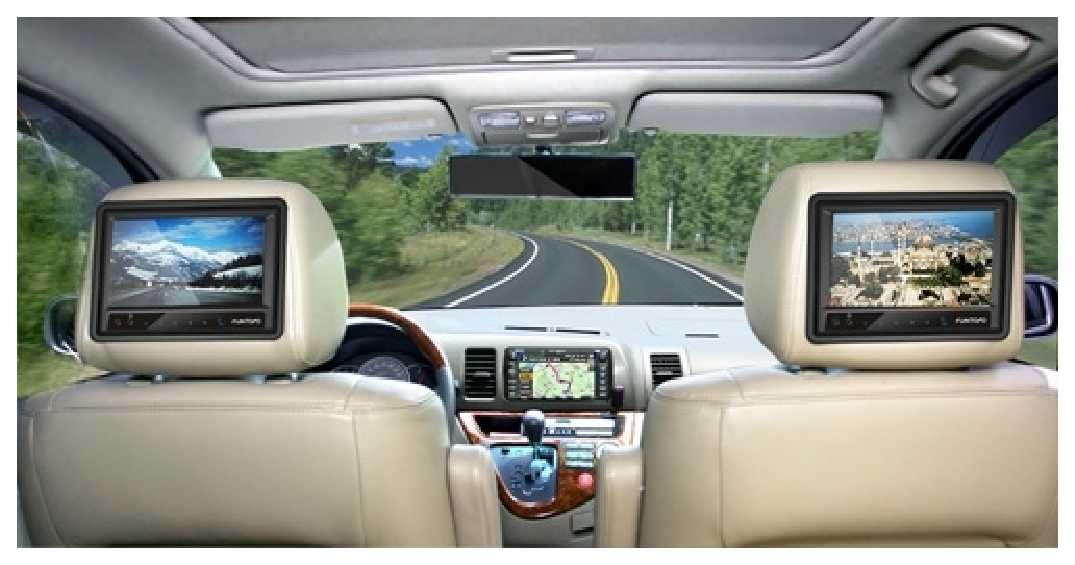
\includegraphics[width=10cm]{car.eps}
            \end{figure}
        \end{itemize}
    \end{frame}

    \begin{frame}[label=principe]
    \frametitle{Principe}
        \begin{itemize}
            \item Mise en évidence de la contention
            \item Problème de partage des composants
            \item Répartition de bande passante
        \end{itemize}
    \end{frame}

    \begin{frame}[label=architecture]
    \frametitle{Architecture utilisée}
    \begin{columns}
        \begin{column}{0.6\textwidth}
            \begin{itemize}
                \item Intel Core i3
                \item Quatre c\oe urs logiques
                \item Trois niveaux de cache
                \item L3 et bus partagés
                \item Isolation des CPUs
            \end{itemize}
        \end{column}
        \begin{column}{0.6\textwidth}
            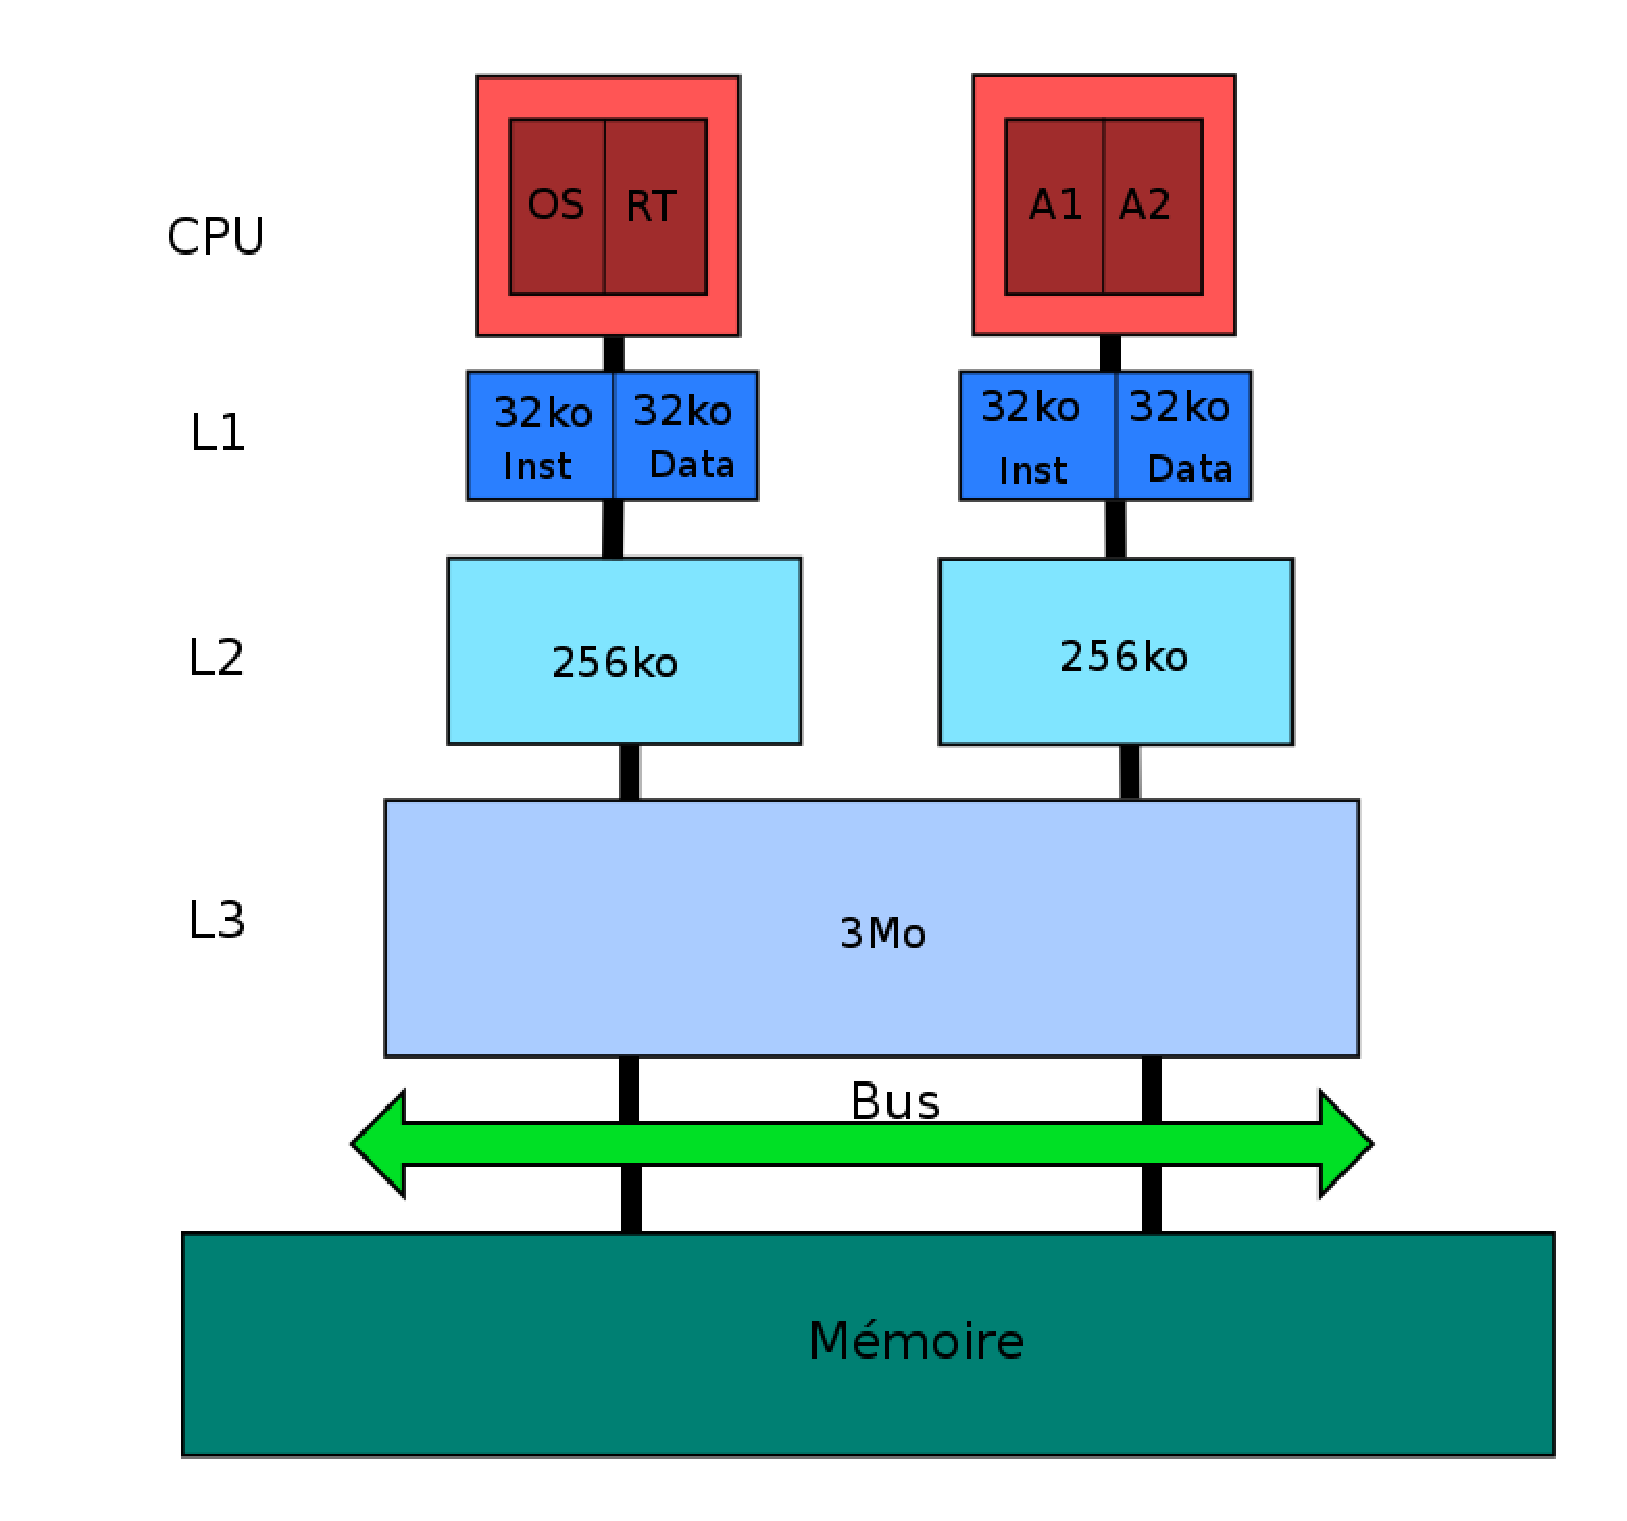
\includegraphics[width=6.5cm]{doc/psar_archi.eps}
        \end{column}
    \end{columns}
    \end{frame}

    \begin{frame}[label=wrapper]
    \frametitle{Wrapper: Mesures des performances}
    \begin{columns}
        \begin{column}{0.6\textwidth}
            \begin{itemize}
                \item Que mesurer?
                \item Librairie PAPI: options et évènements
                \item Clouer des processus sur les CPUs
            \end{itemize}
        \end{column}
        \begin{column}{0.6\textwidth}
            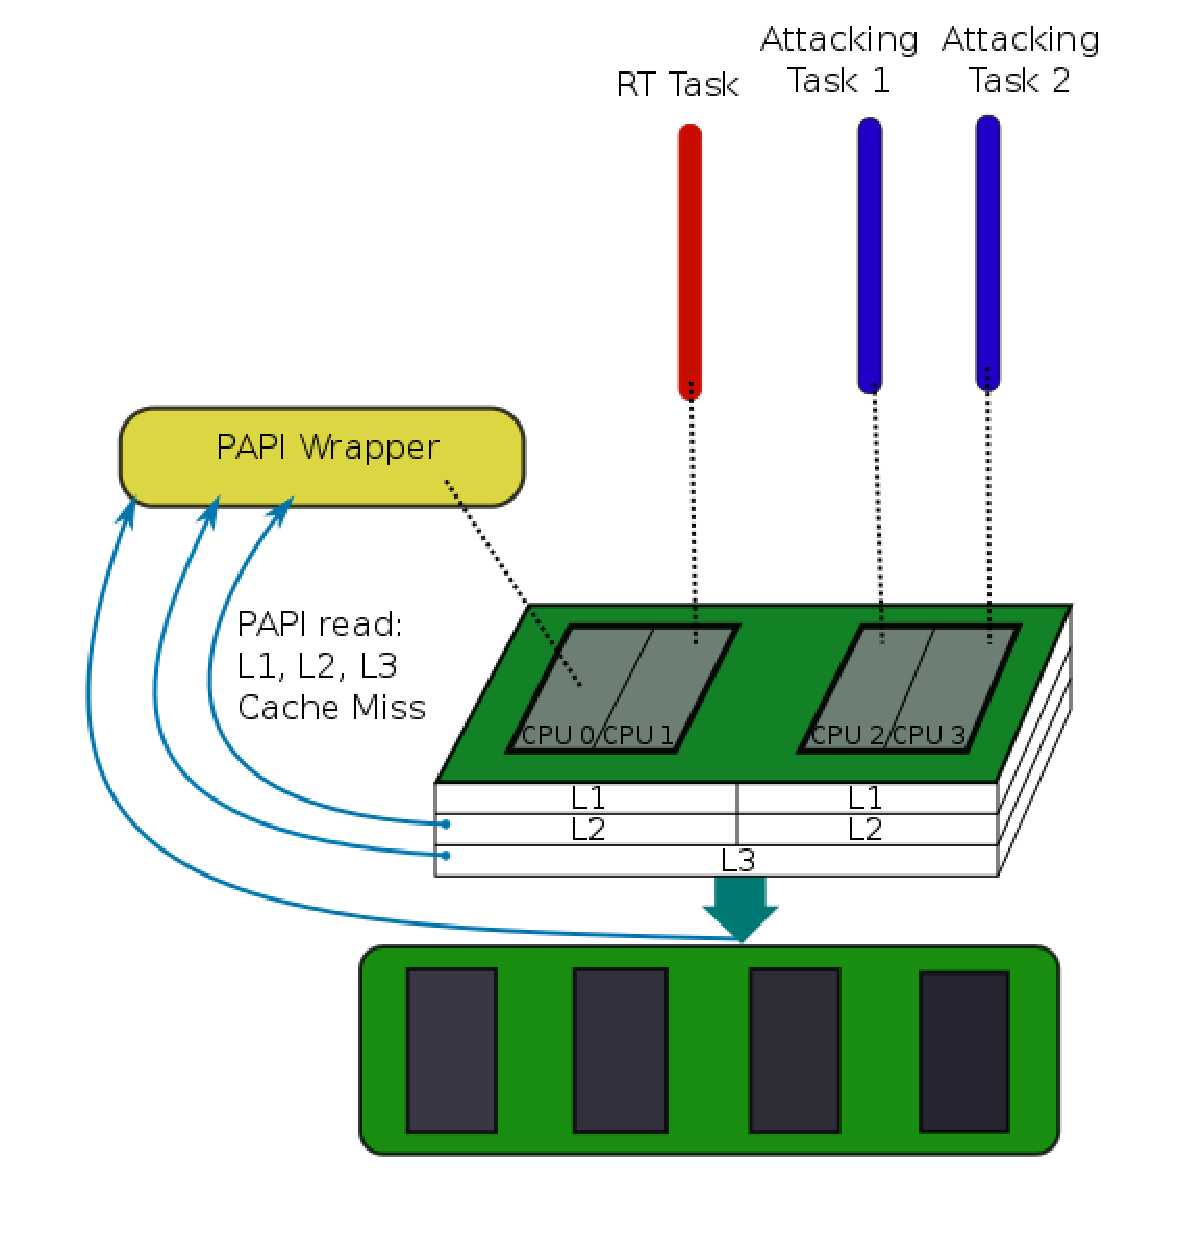
\includegraphics[width=6.5cm]{doc/psar_wrapper.eps}
        \end{column}
    \end{columns}
    \end{frame}

    \begin{frame}[label=temps-reel]
    \frametitle{Tâche temps-réel}
    \begin{itemize}
        \item Tableaux statiques de grande taille
        \item Parcours aléatoire (préfetching)
        \item Regarde si son échéance est satisfaite
            \begin{figure}
                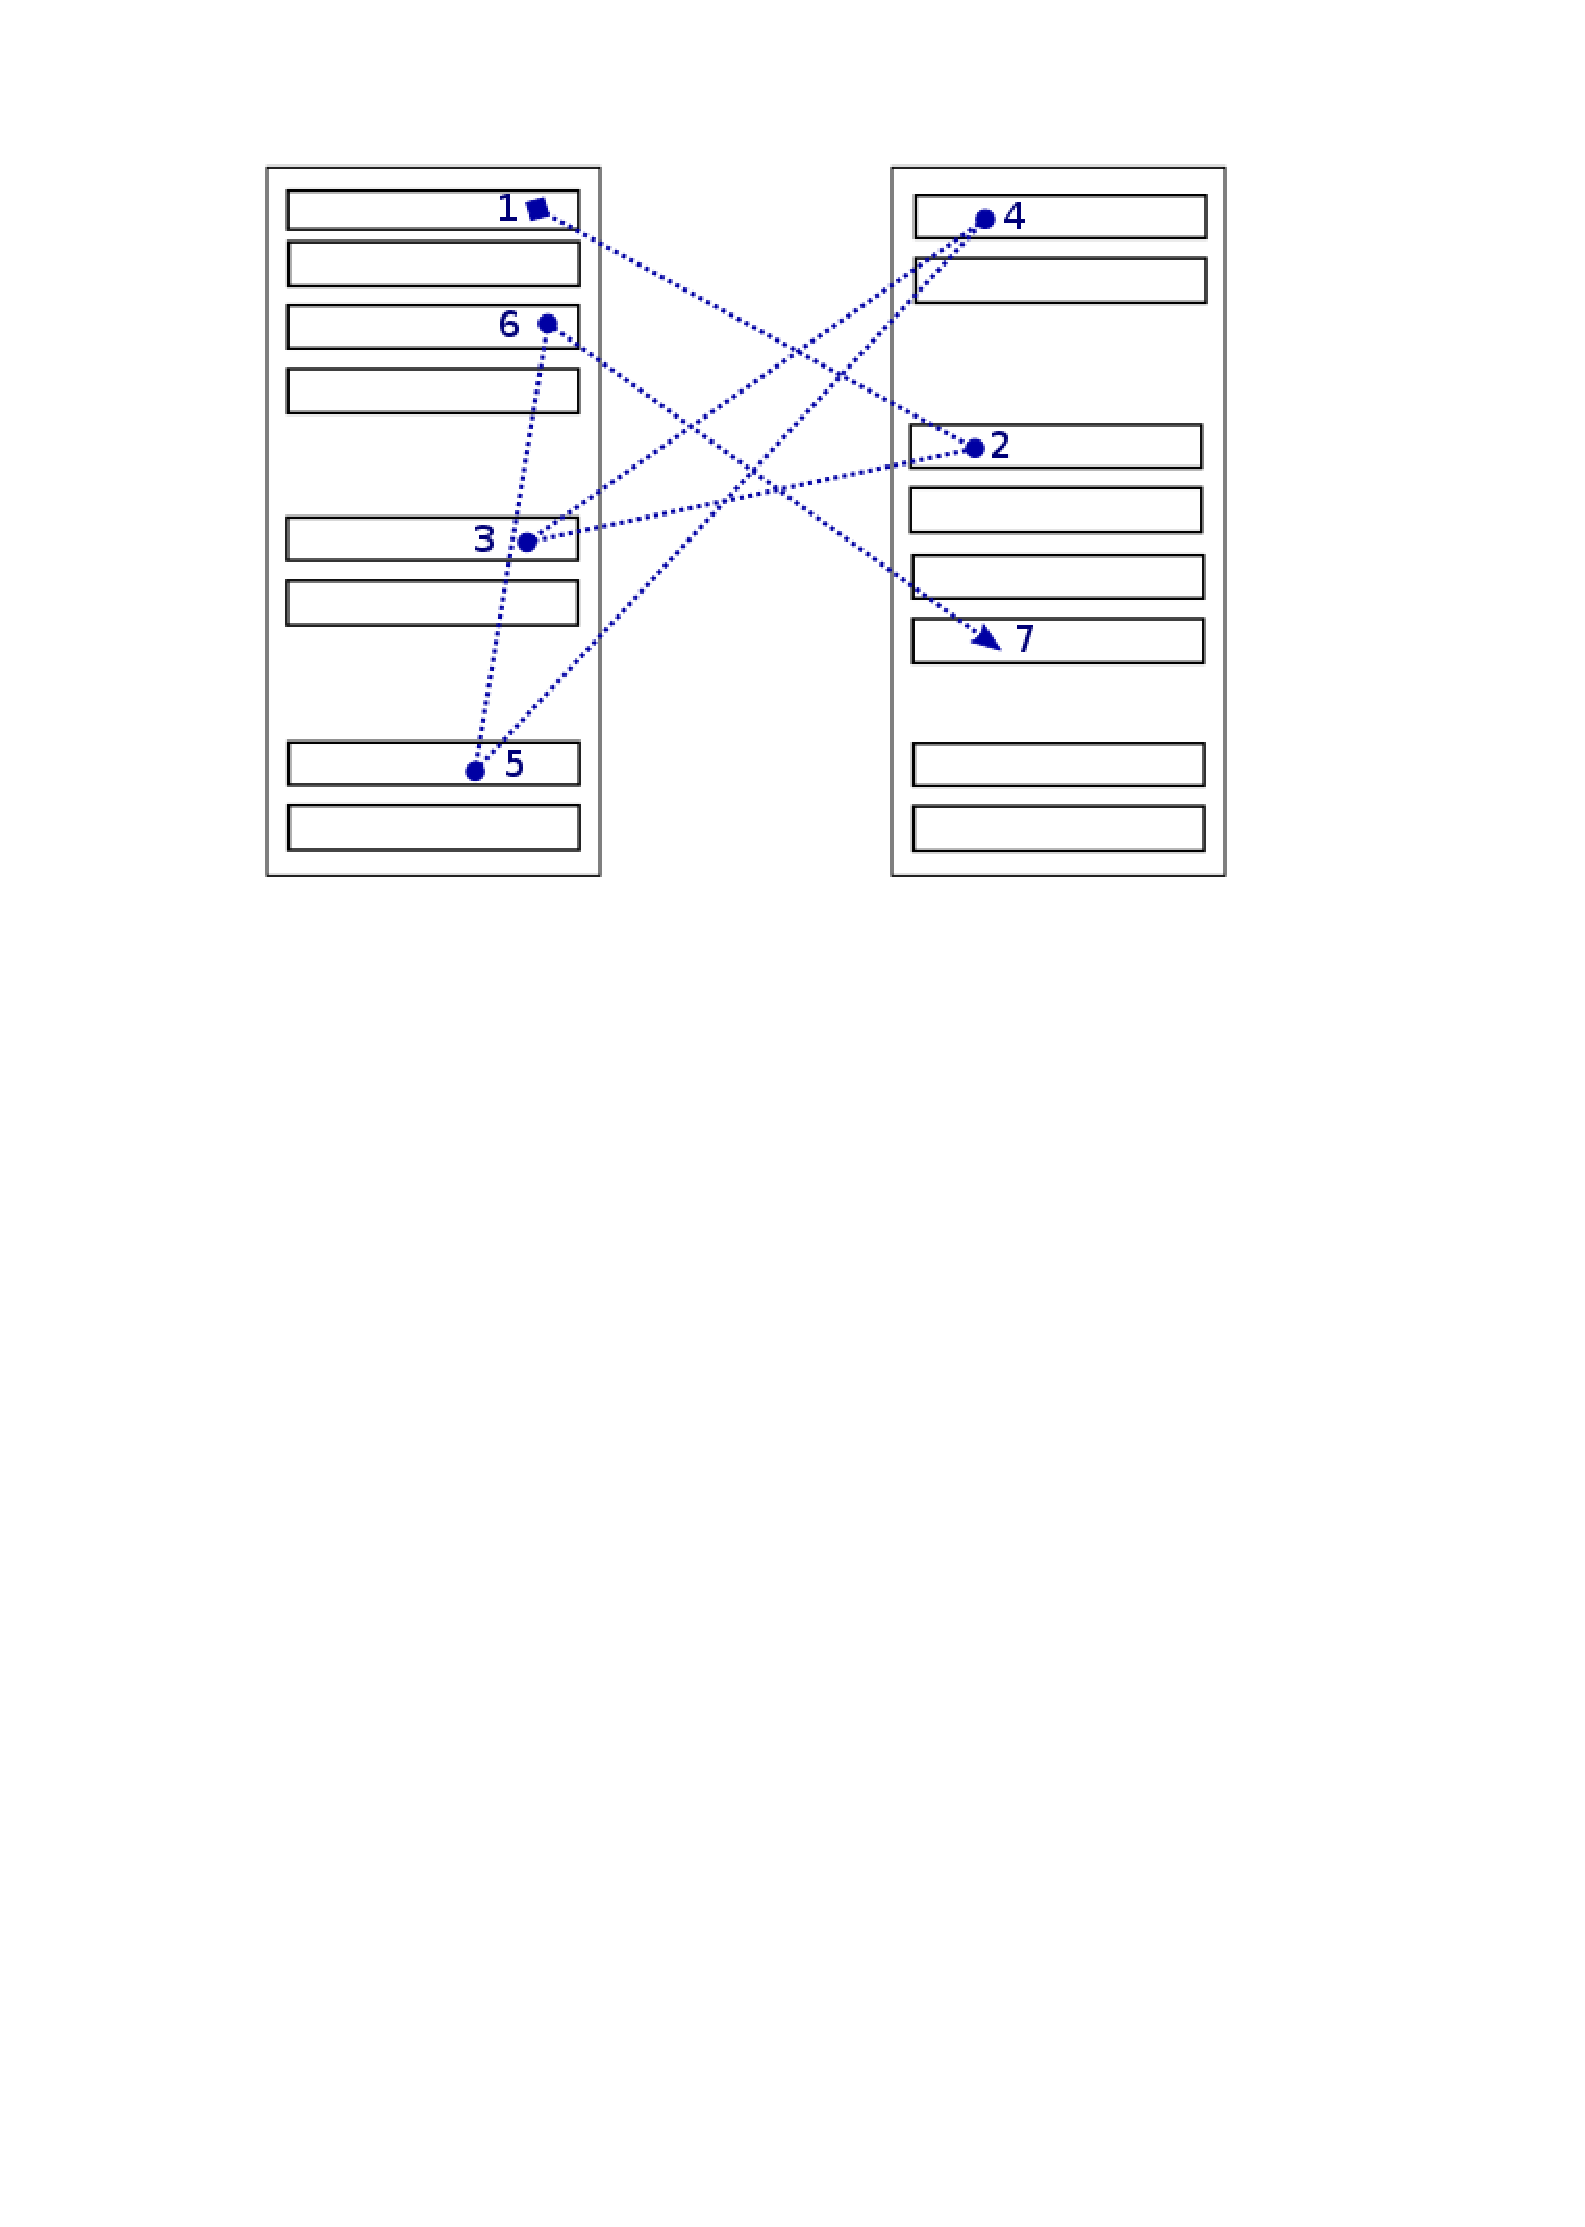
\includegraphics[width=8cm]{doc/psar_rt.eps}
            \end{figure}
    \end{itemize}
    \end{frame}
    
    \begin{frame}[label=attaquants]
        \frametitle{Tâches attaquantes}
        \begin{itemize}
            \item Liste dynamique de grande taille
            \item Éléments de la liste: matrices carrées
            \item Itérations aléatoires
        \end{itemize}
        \begin{figure}
            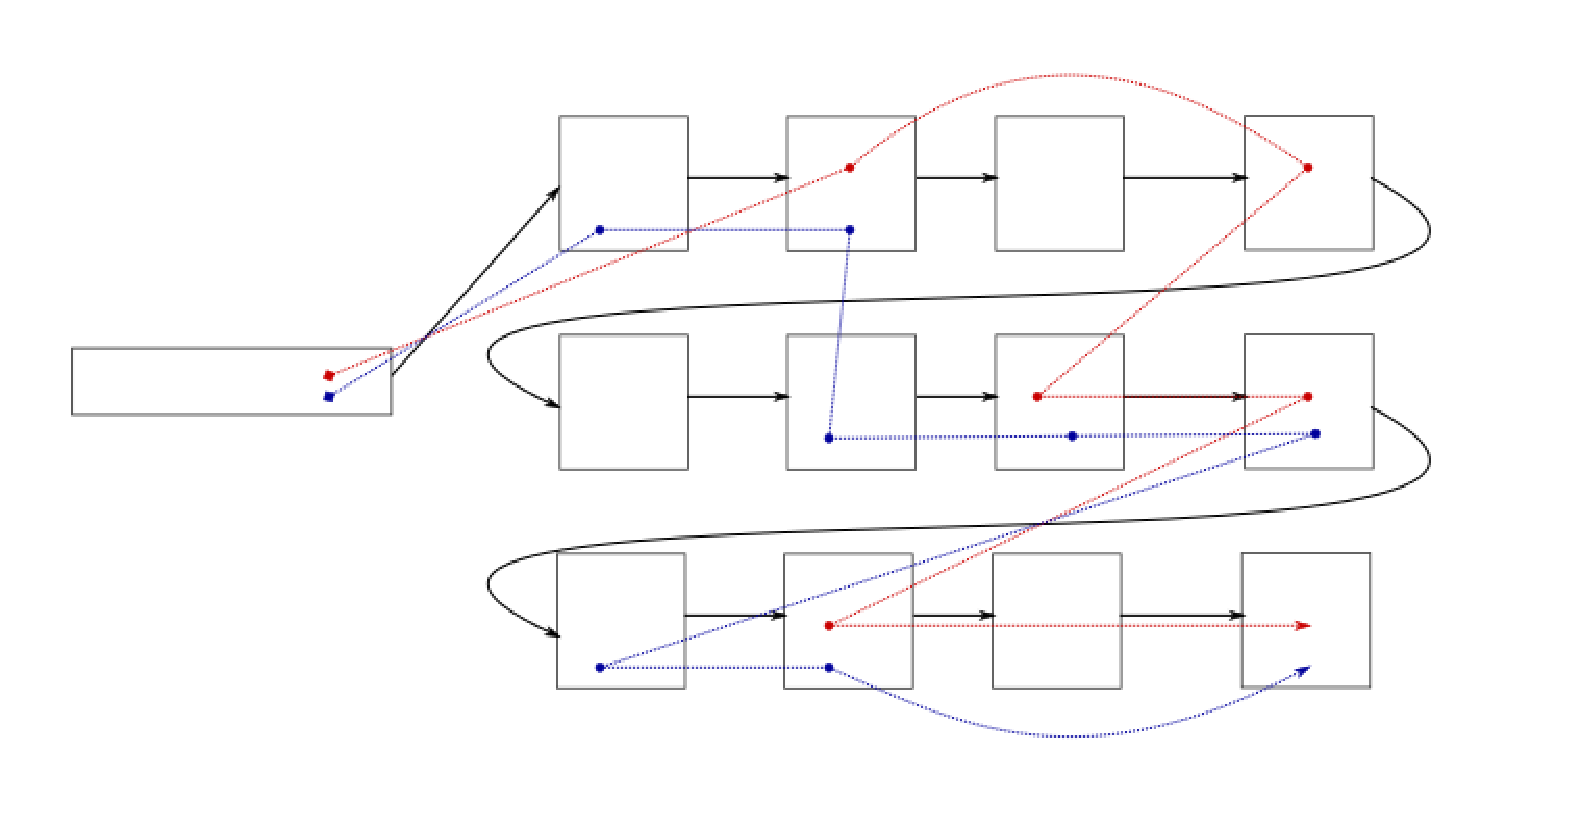
\includegraphics[width=9cm]{doc/psar_attaquants.eps}
        \end{figure}

    \end{frame}
    
    \begin{frame}[label=concurrence]
        \frametitle{Problème de concurrence d'accès}
        \begin{itemize}
            \item Augmentation du temps d'exécution
            \item Augmentation du nombre de cache MISS
        \end{itemize}
        \begin{figure}
            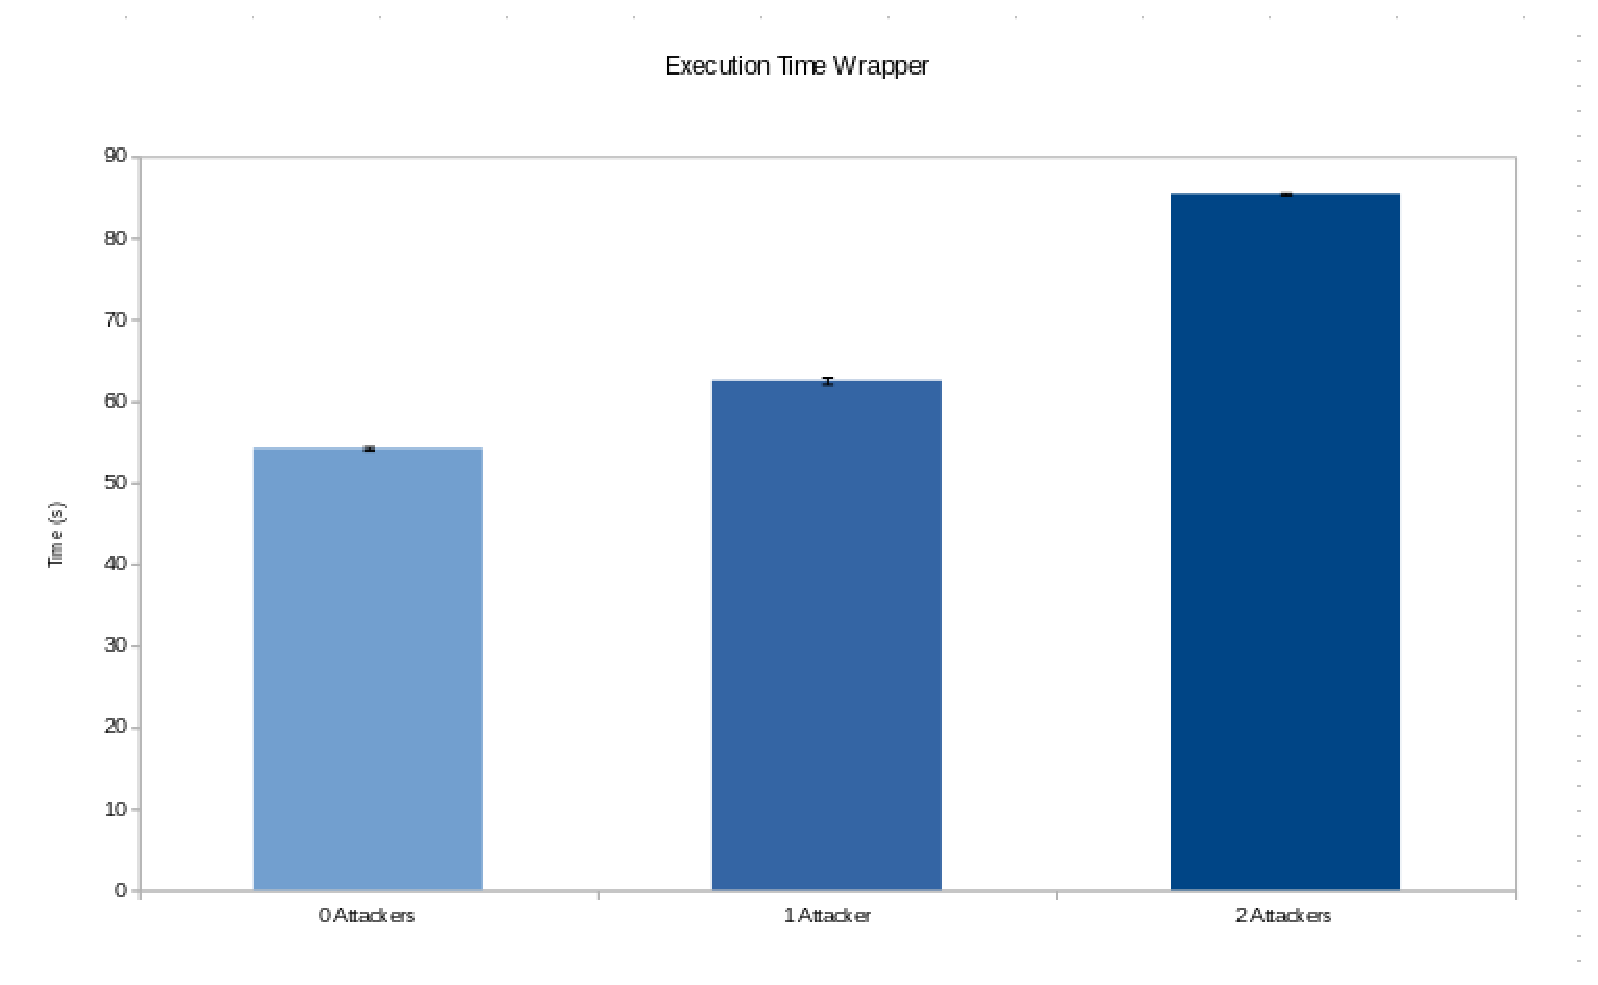
\includegraphics[width=9cm]{doc/graphes/benchmark_wrapper_performance.eps}
        \end{figure}
    \end{frame}

    \begin{frame}[label=sous-reservation]
        \frametitle{Sous réservation de BP mémoire}
        \begin{itemize}
            \item Temps d'exécution tâche temps-réel
            \item Répartition équitable de BP
            \item Compteurs globaux
        \end{itemize}
        \begin{figure}
            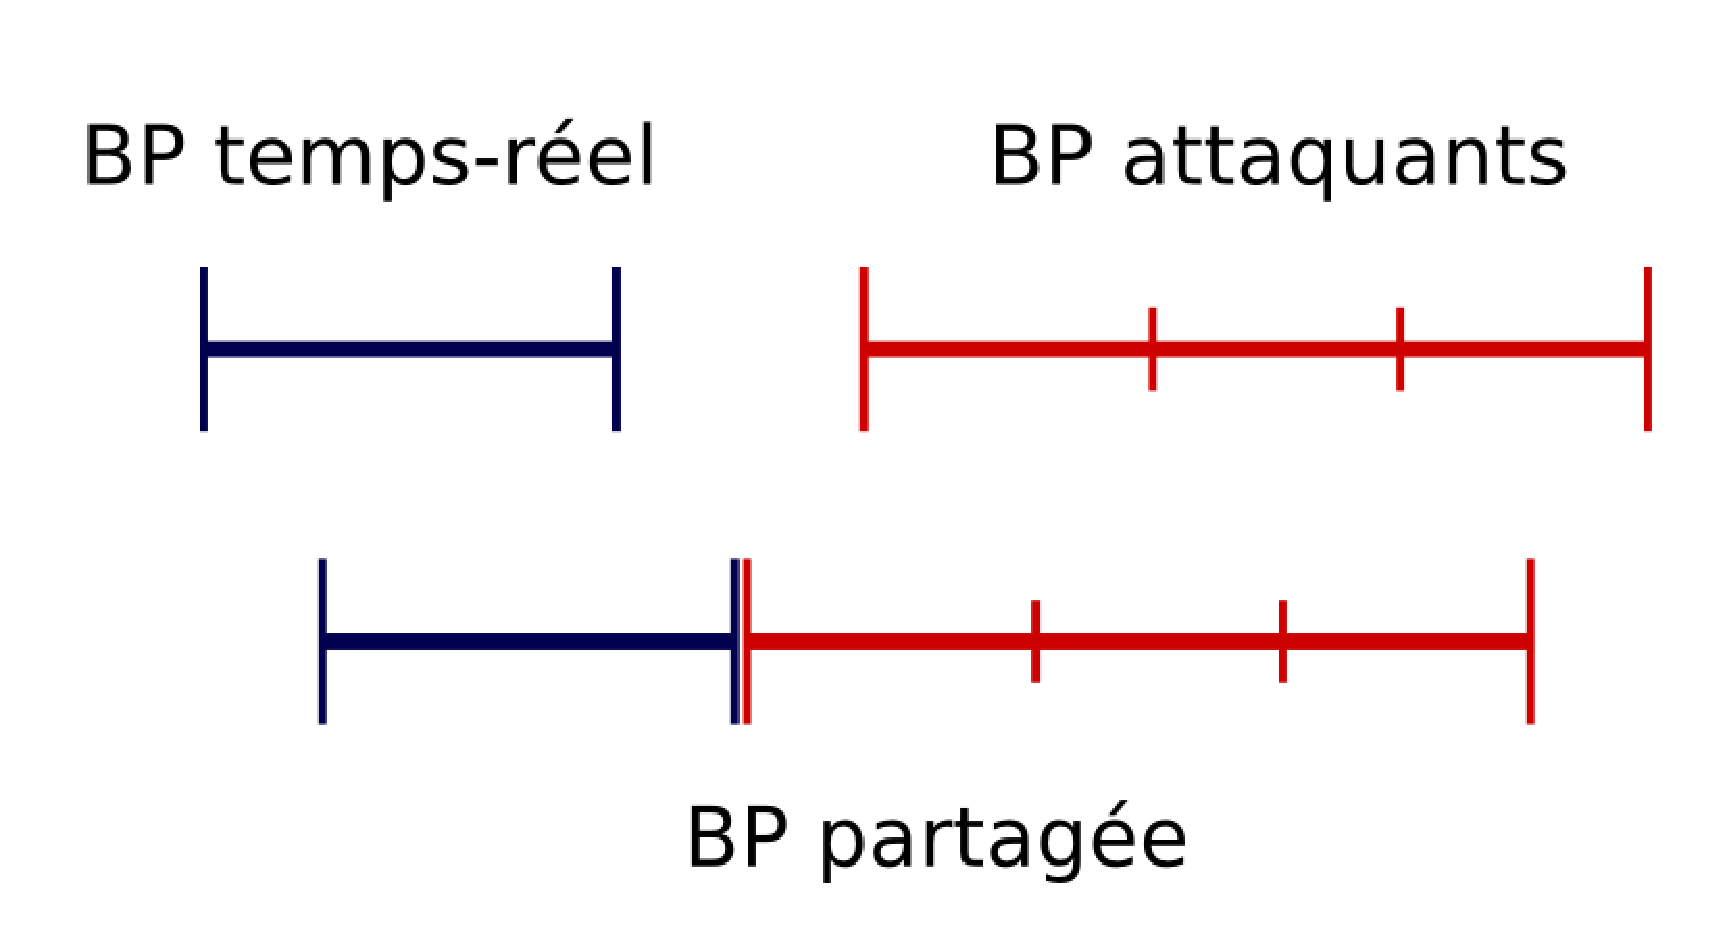
\includegraphics[width=6cm]{doc/schema_bp.eps}
        \end{figure}
    \end{frame}
    
    \begin{frame}[label=mecanisme]
        \frametitle{Mécanisme d'arrêt: solution en mode utilisateur}
        \begin{columns}
            \begin{column}{0.6\textwidth}
                \begin{itemize}
                    \item Signaux POSIX
                    \item Attaquants arrêtés
                    \item Timer réveille le mécanisme
                \end{itemize}
            \end{column}
            \begin{column}{0.8\textwidth}
                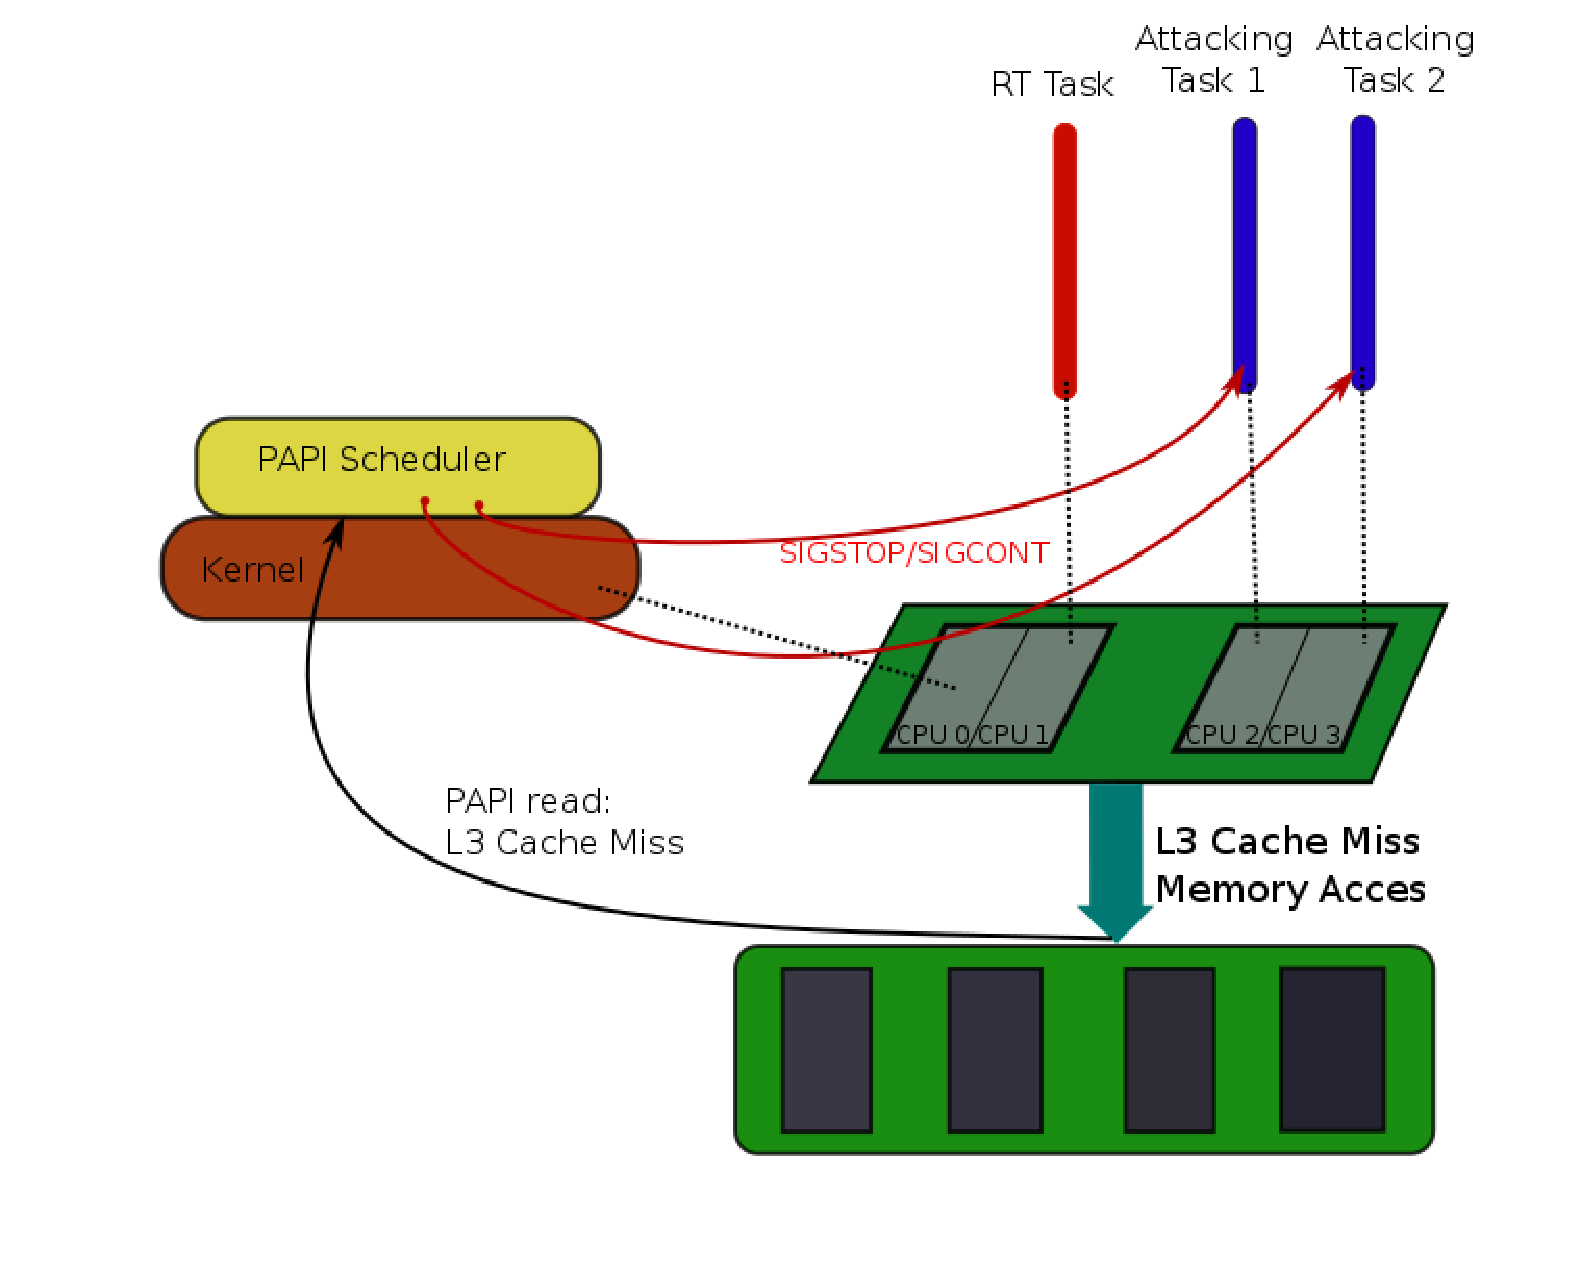
\includegraphics[width=6.5cm]{doc/papi_scheduler.eps}
            \end{column}
        \end{columns}
    \end{frame}

    \begin{frame}[label=resultats]
        \frametitle{Résultats (1)}
        \begin{itemize}
            \item Mise en évidence de la contention mémoire
            \item Efficacité du mécanisme d'arrêt
                \begin{itemize}
                    \item Introduction de latence (coût du mécanisme)
                    \item Stabilisation du temps d'exécution
                    \item Diminution du taux des MISS
                \end{itemize}
        \end{itemize}
    \end{frame}

    \begin{frame}[label=wrapper_vs_scheduler]
        \frametitle{Résultats (2): comparaison}
        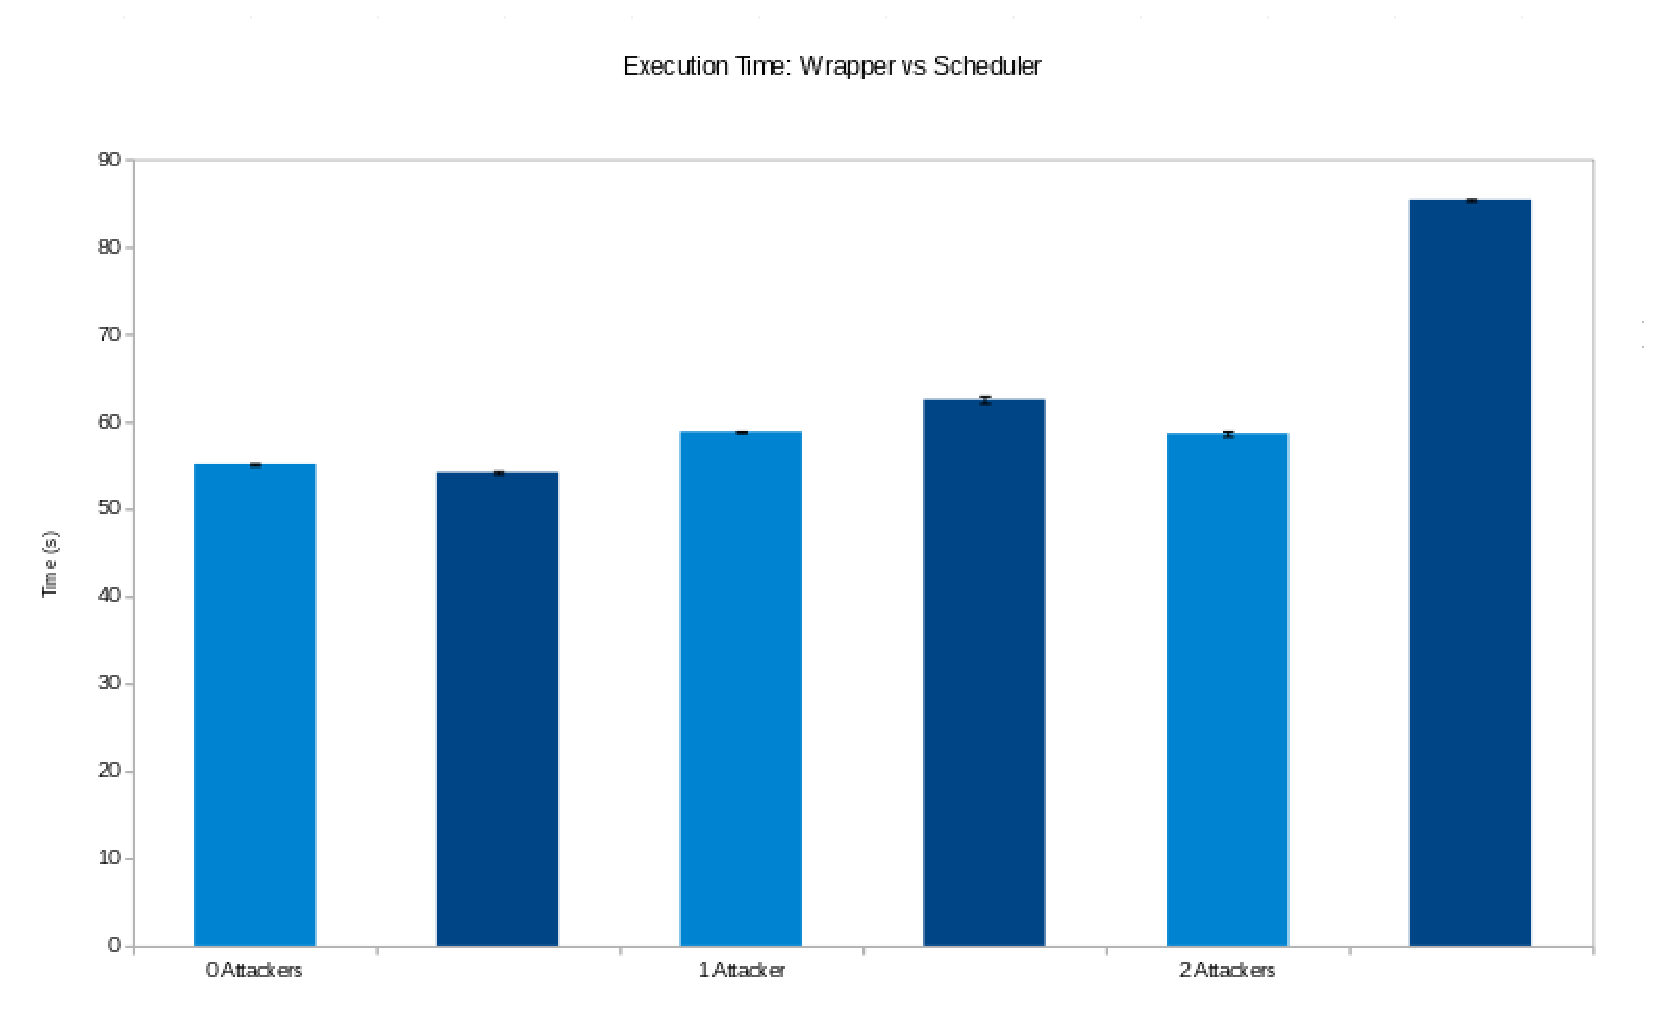
\includegraphics[width=10cm]{doc/graphes/benchmark_1_performance.eps}
    \end{frame}

    \begin{frame}[label=conclusion]
        \frametitle{Conclusion}
        \begin{itemize}
            \item Mise en évidence du problème
            \item Developpement d'une plateforme de test
            \item Mesures de l'efficacité et dimensionnement:
                \begin{itemize}
                    \item Temps d'exécution borné
                    \item Accès concurrents à la mémoire
                \end{itemize}
        \end{itemize}
    \end{frame}

    \begin{frame}[label=demo]
        \frametitle{DEMO}
        \begin{center}
            
\includegraphics[width=5cm]{kid.eps}
        \end{center}
    \end{frame}

\end{document}
